\chapter{Model Training Loss}
\label{appendix:training-loss}

\begin{figure}[ht]
    \centering
    \begin{subfigure}[b]{0.49\textwidth}
        \centering
        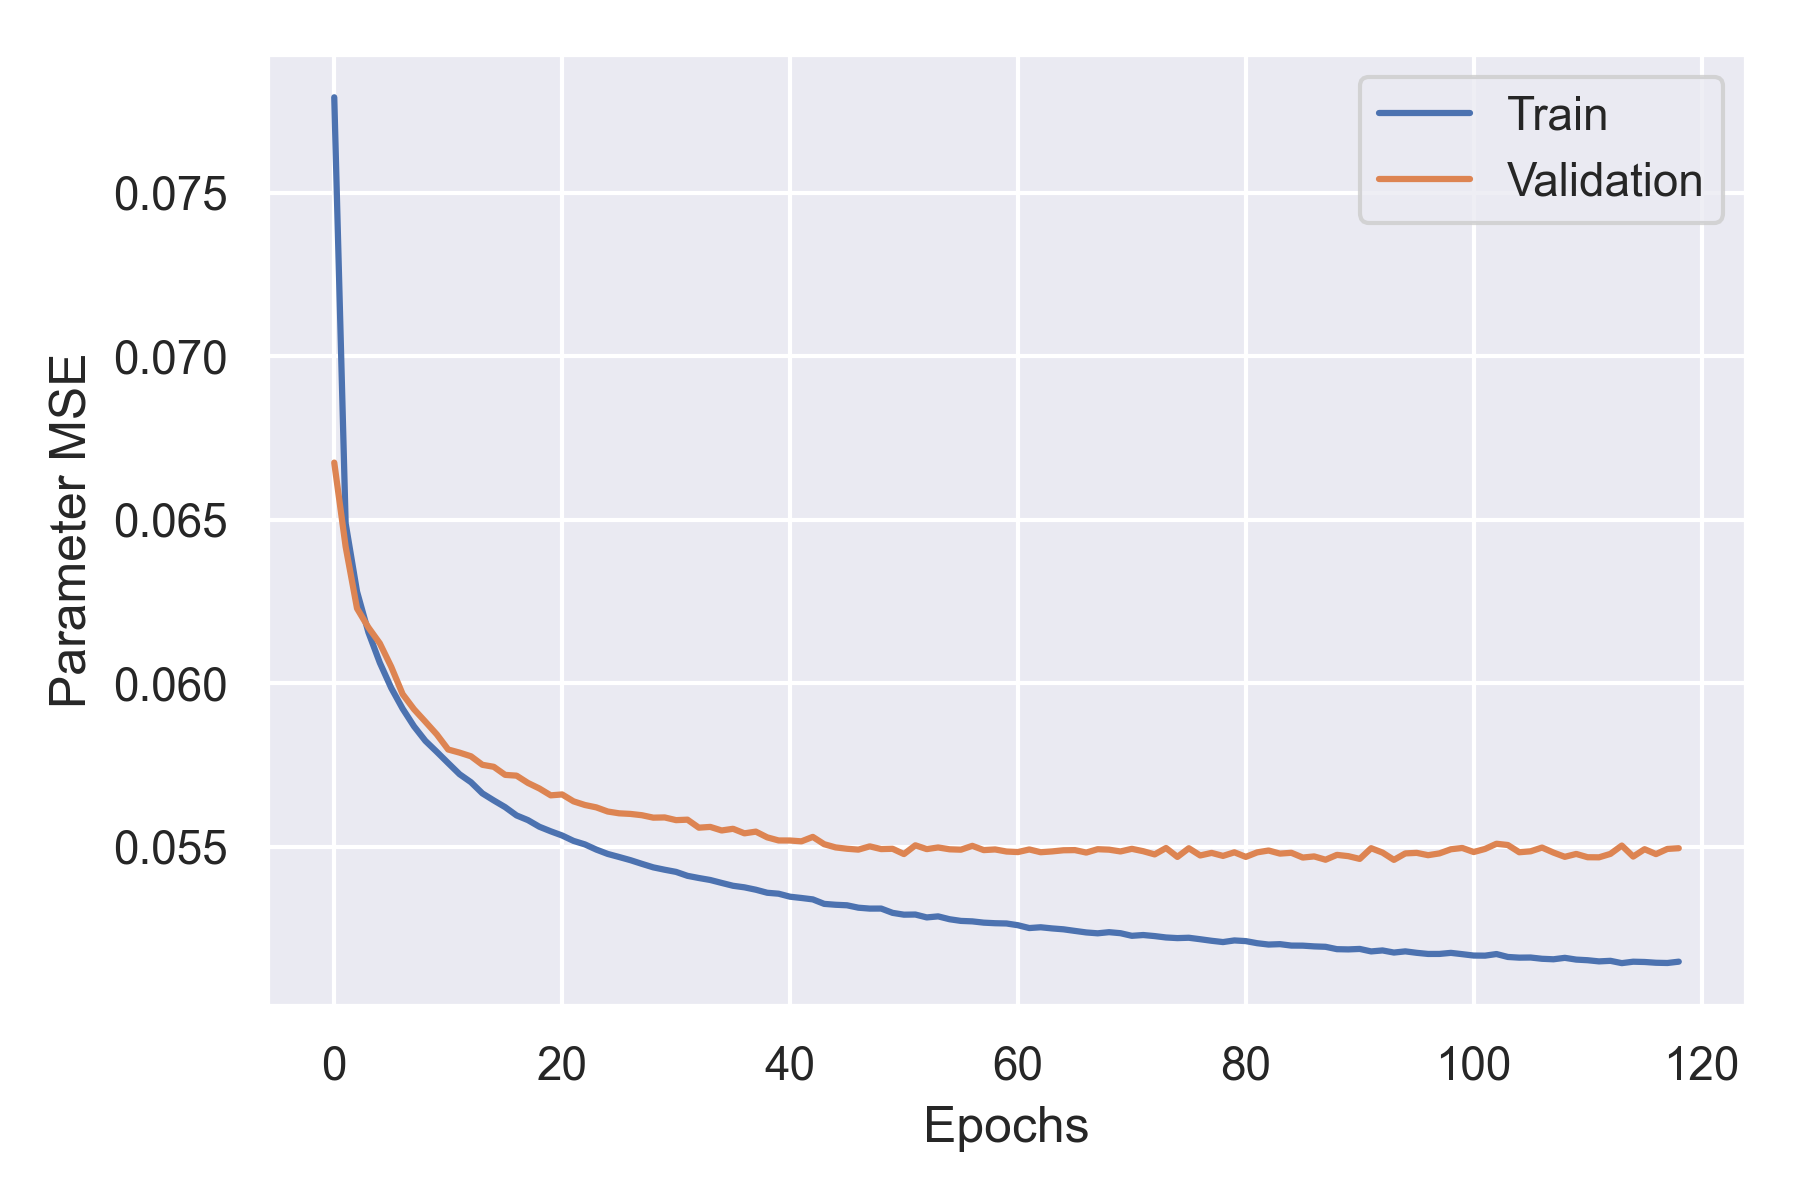
\includegraphics[width=\textwidth]{figures/inverse-synth/loss-plots/mlp-mfcc.png}
        \caption{MLP}
    \end{subfigure}
    \begin{subfigure}[b]{0.49\textwidth}
        \centering
        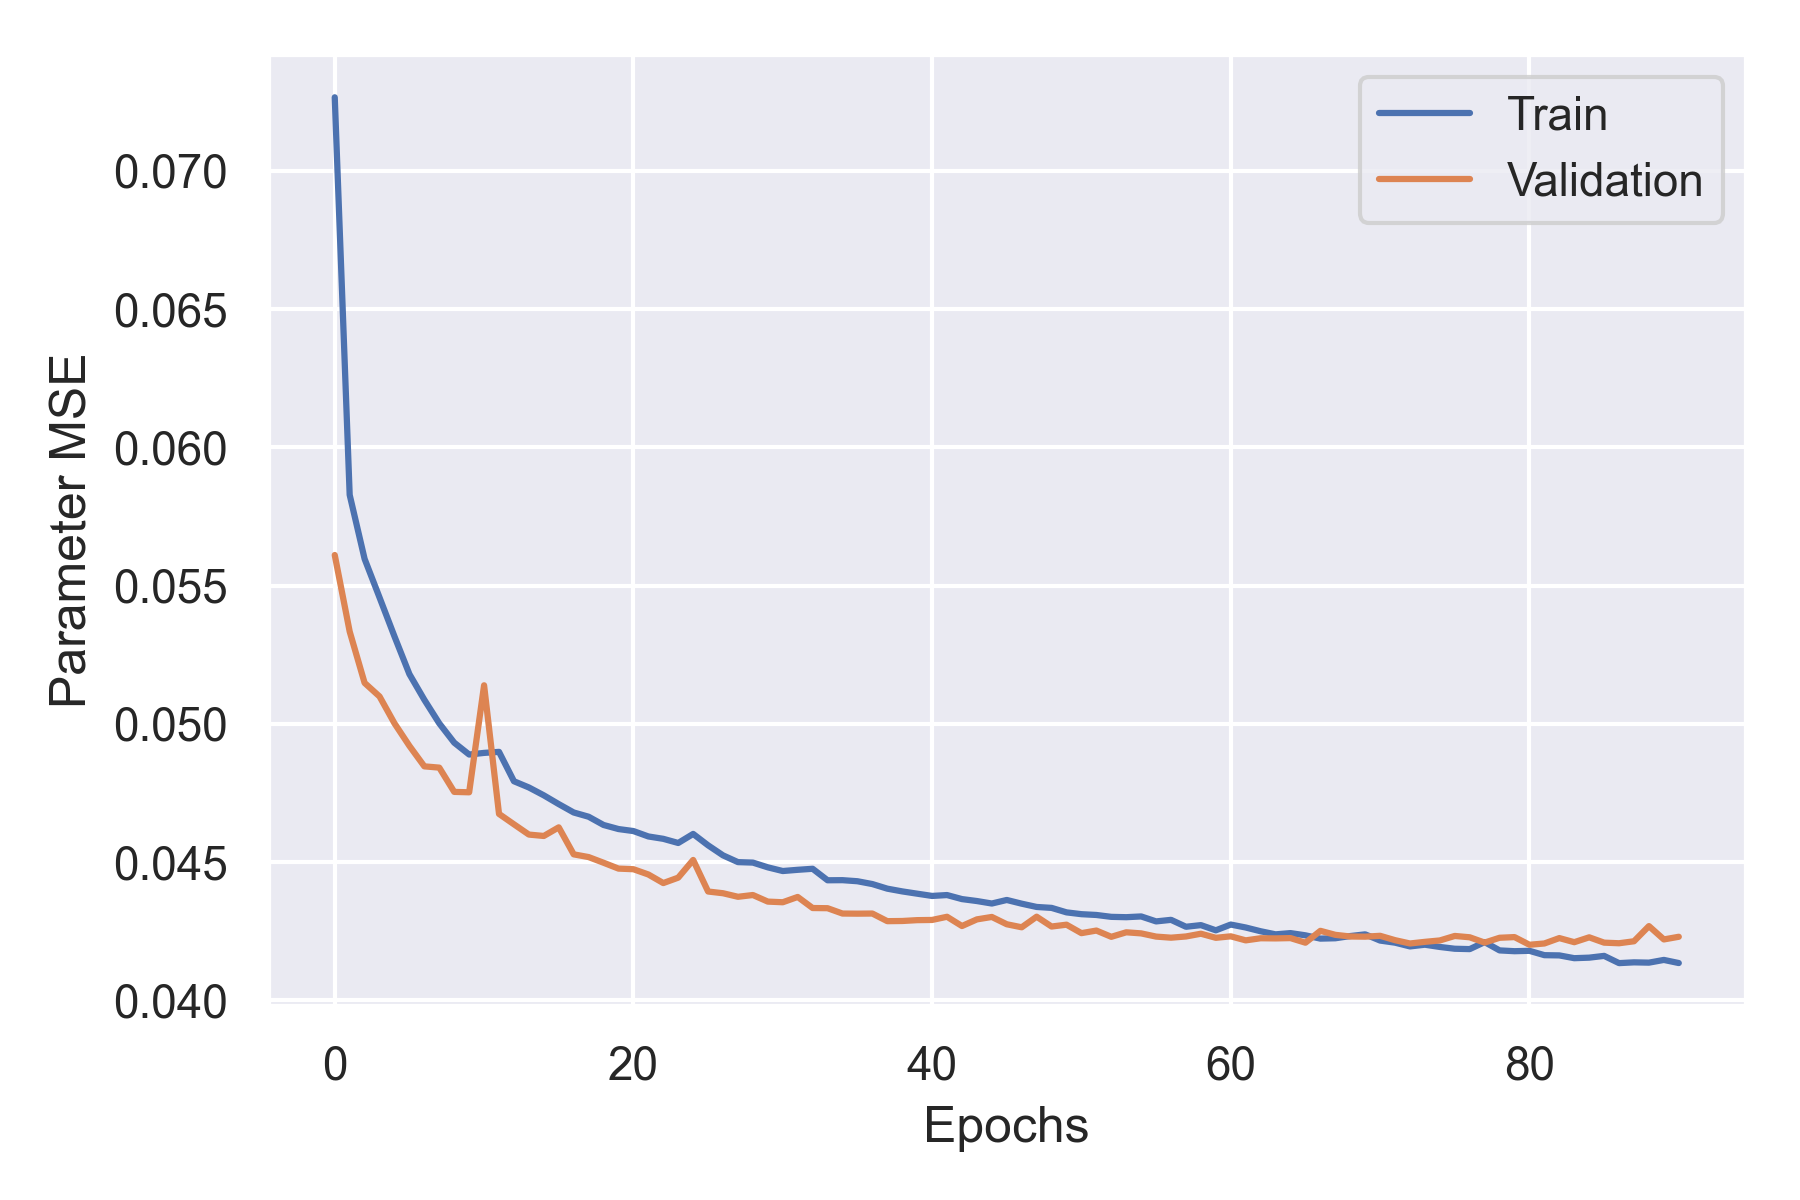
\includegraphics[width=\textwidth]{figures/inverse-synth/loss-plots/lstm-mfcc.png}
        \caption{LSTM}
    \end{subfigure}
    
    \vspace{1cm}
    
    \begin{subfigure}[b]{0.49\textwidth}
        \centering
        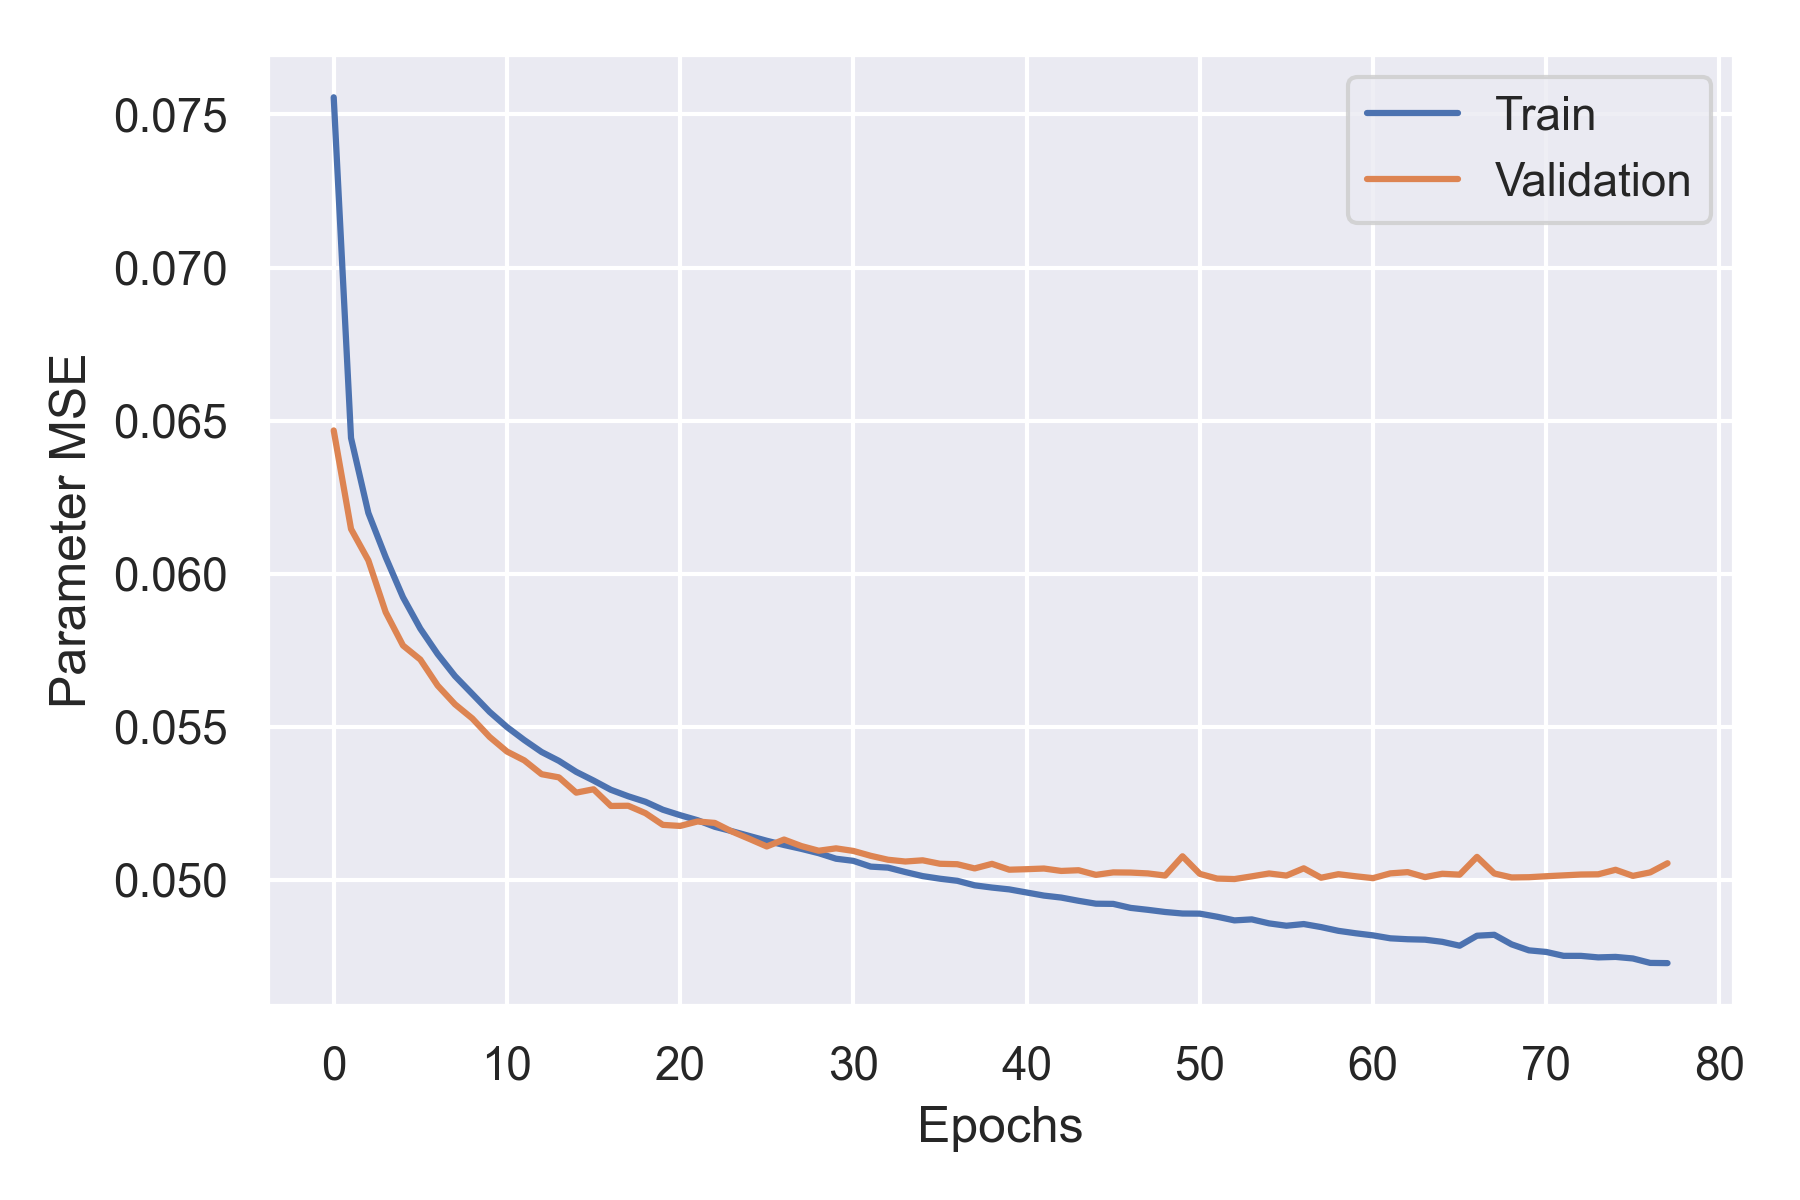
\includegraphics[width=\textwidth]{figures/inverse-synth/loss-plots/bilstm-mfcc.png}
        \caption{LSTM++}
    \end{subfigure}
    \begin{subfigure}[b]{0.49\textwidth}
        \centering
        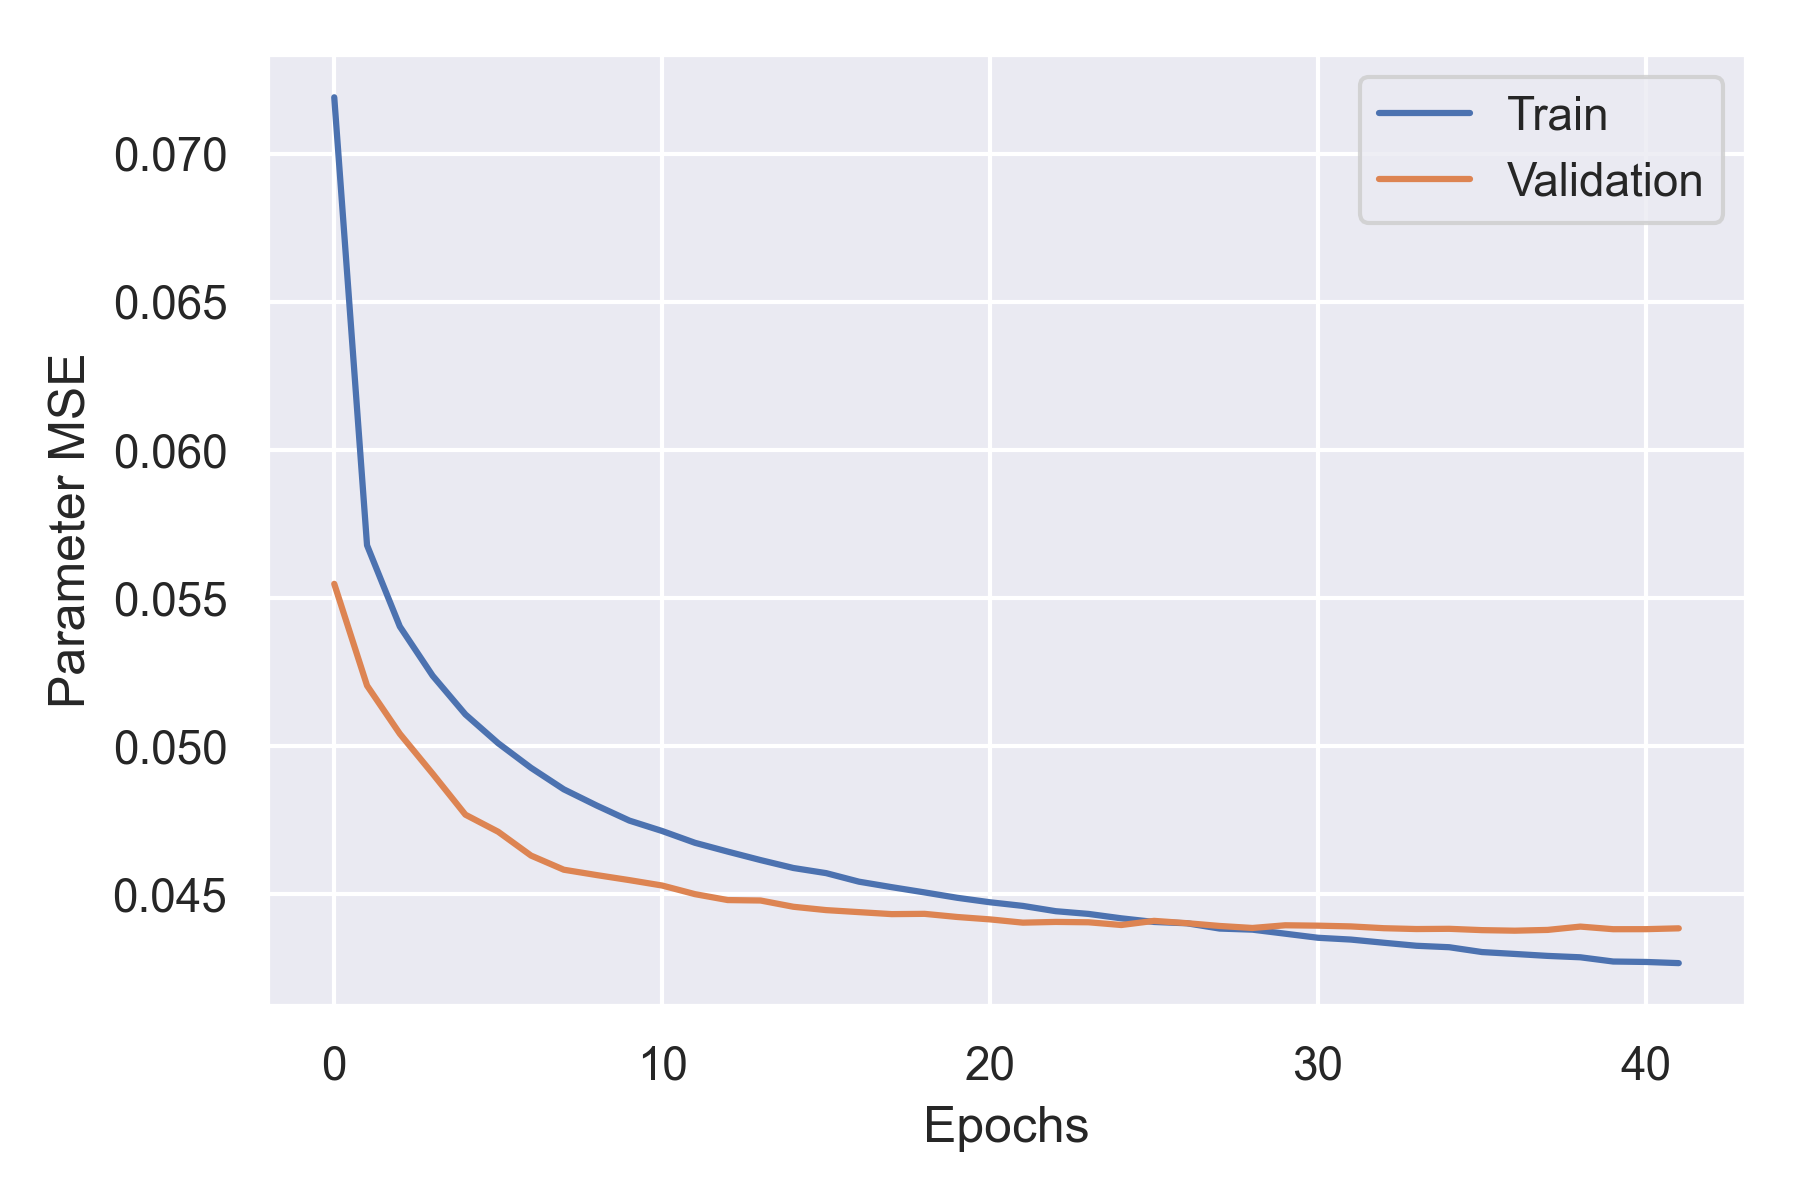
\includegraphics[width=\textwidth]{figures/inverse-synth/loss-plots/cnn-mfcc.png}
        \caption{CNN}
    \end{subfigure}
    \caption{MFCC Model Training and Validation Loss Plots}
\end{figure}

\begin{figure}[t]
    \centering
    \begin{subfigure}[b]{0.49\textwidth}
        \centering
        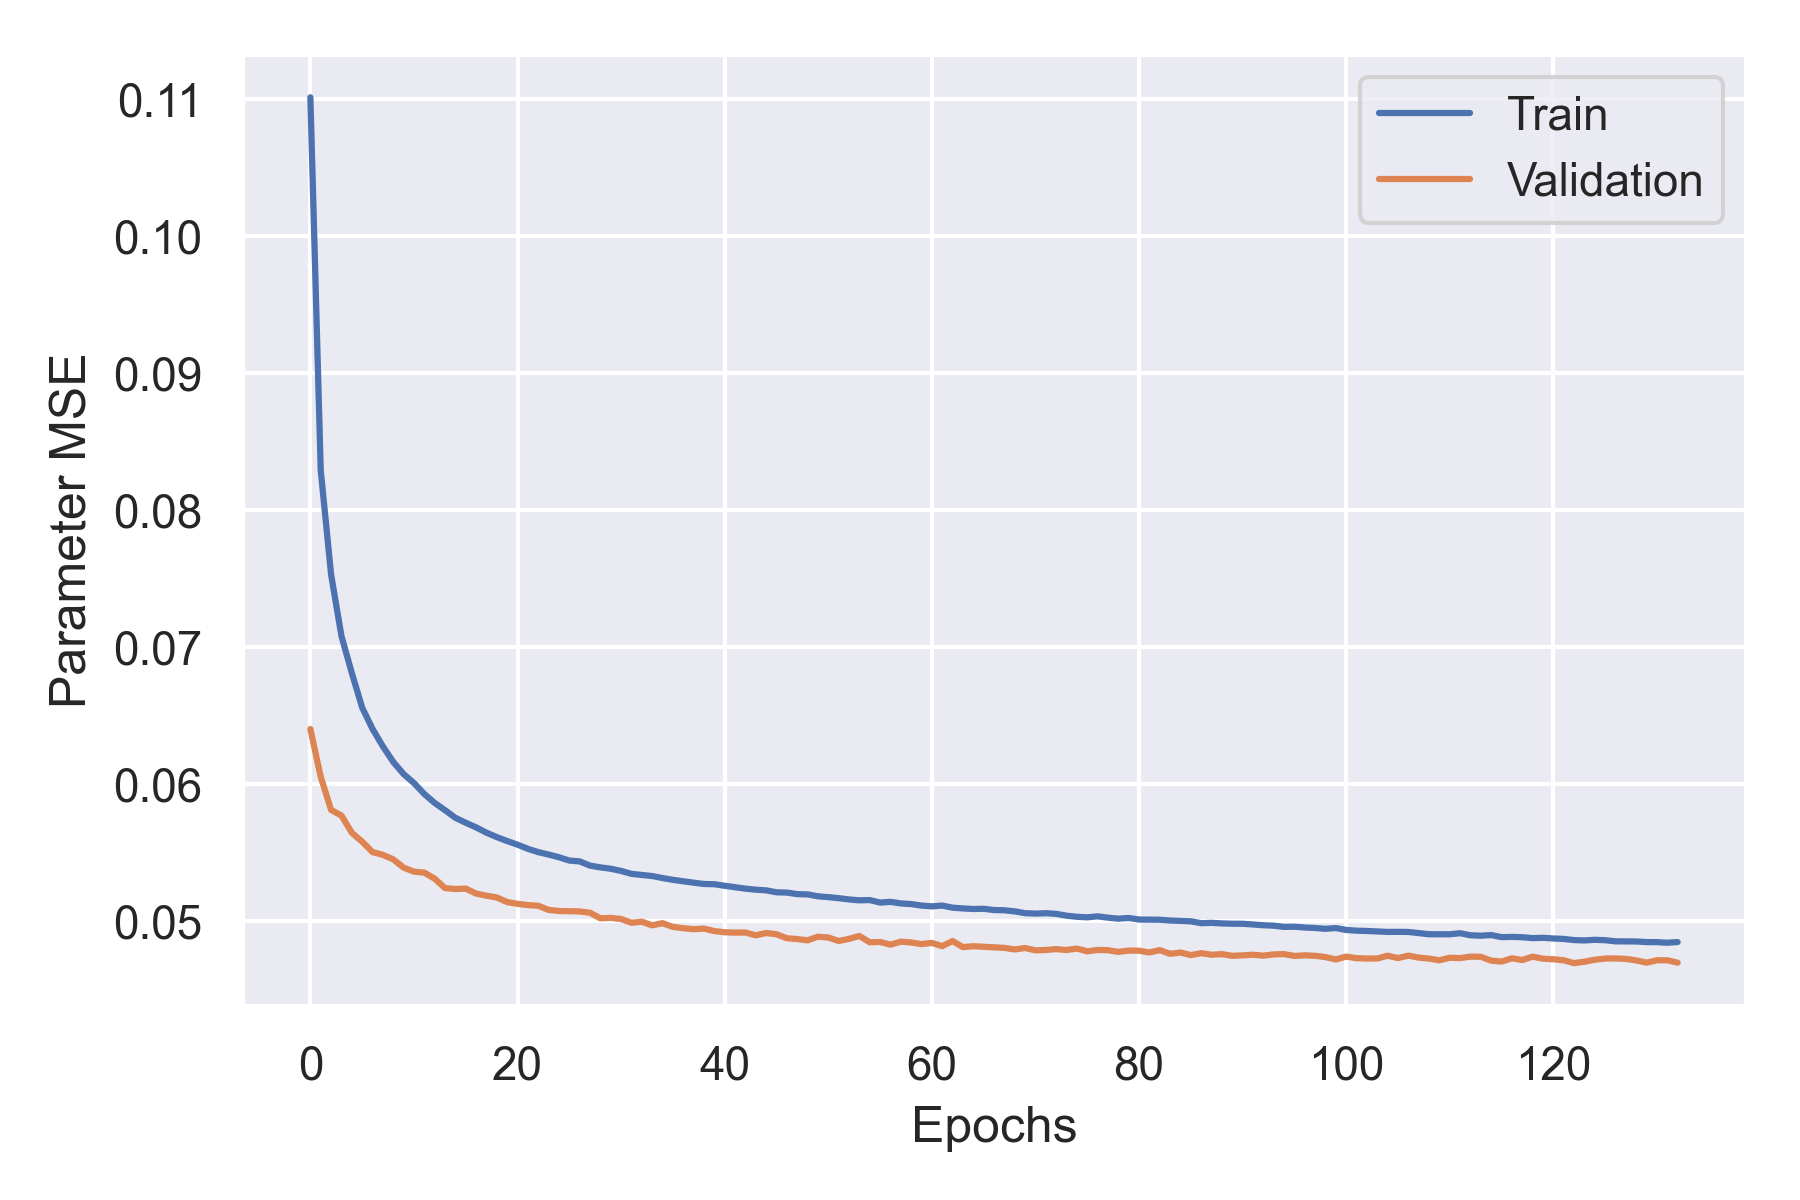
\includegraphics[width=\textwidth]{figures/inverse-synth/loss-plots/mlp-mel.png}
        \caption{MLP}
    \end{subfigure}
    \begin{subfigure}[b]{0.49\textwidth}
        \centering
        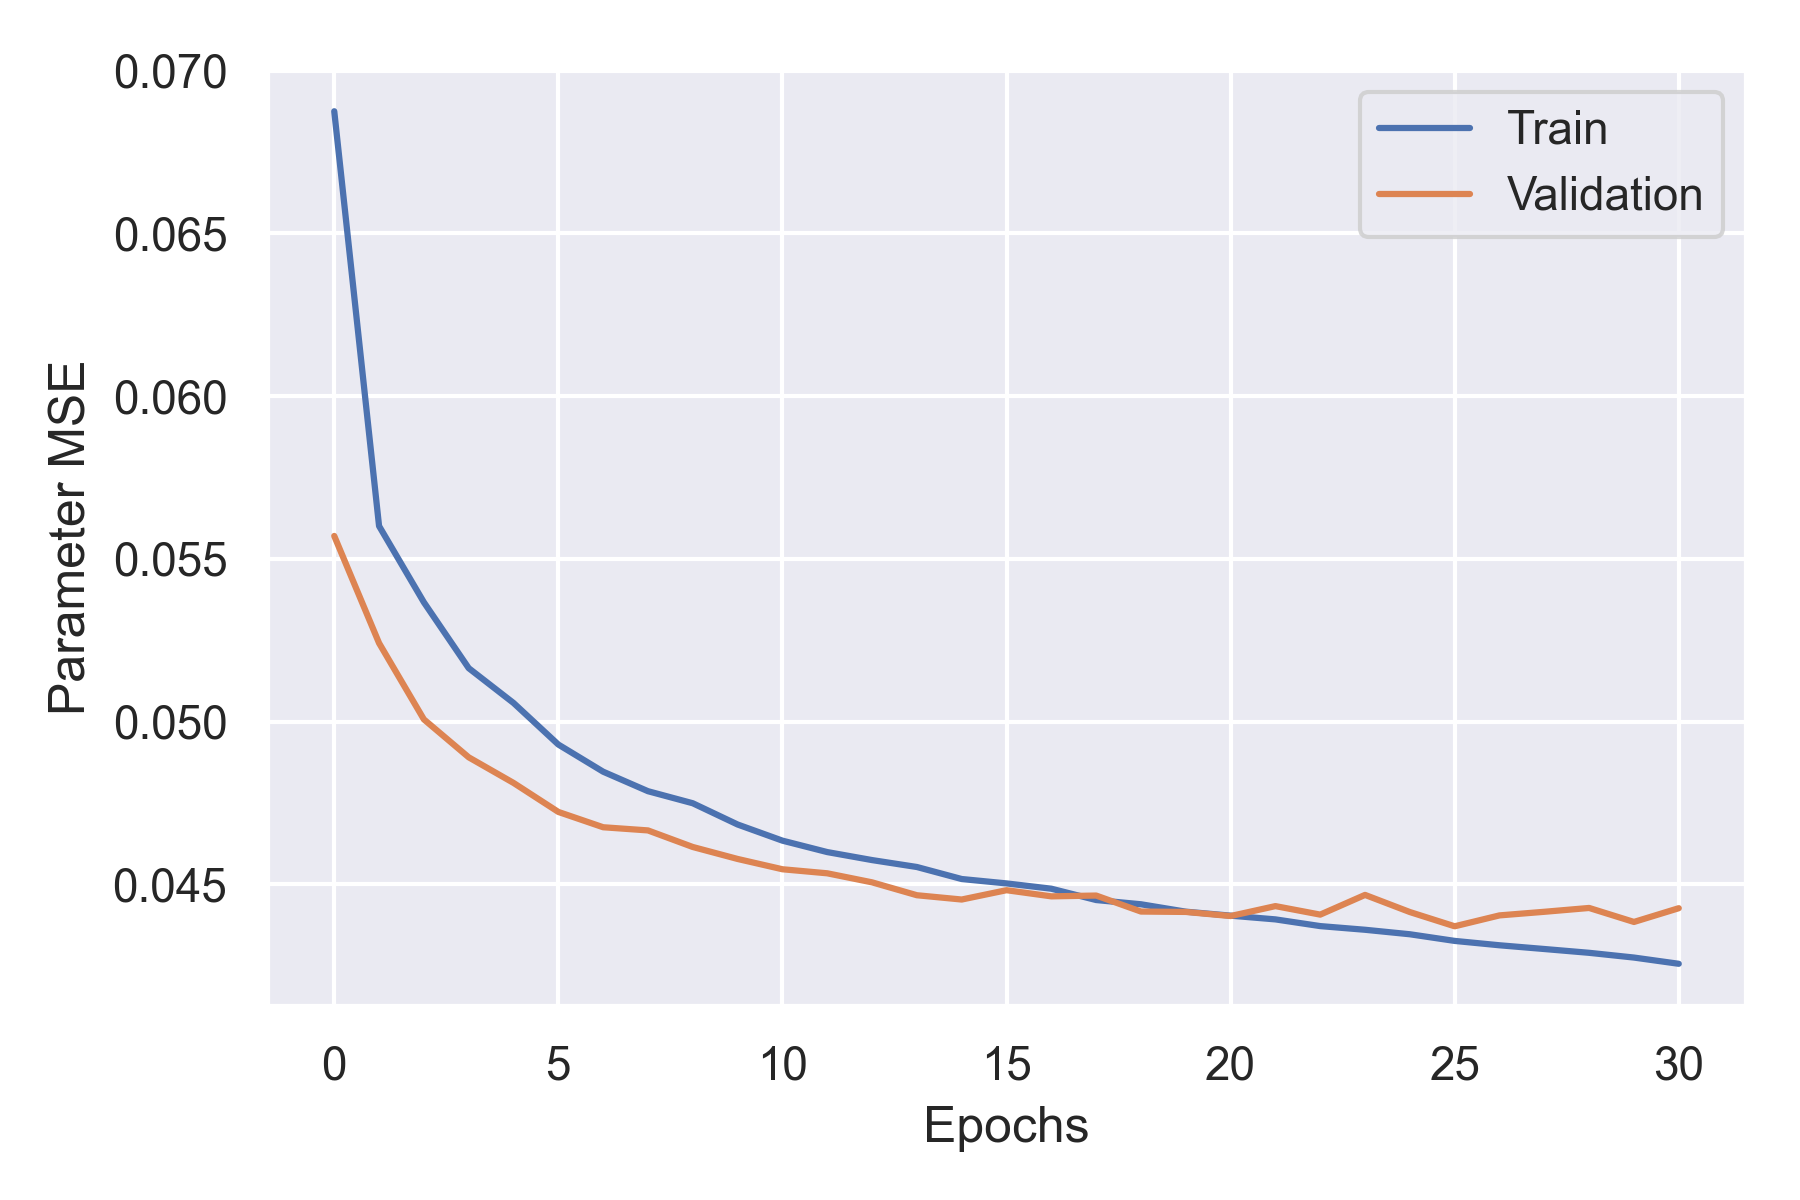
\includegraphics[width=\textwidth]{figures/inverse-synth/loss-plots/lstm-mel.png}
        \caption{LSTM}
    \end{subfigure}
    
    \vspace{1cm}
    
    \begin{subfigure}[b]{0.49\textwidth}
        \centering
        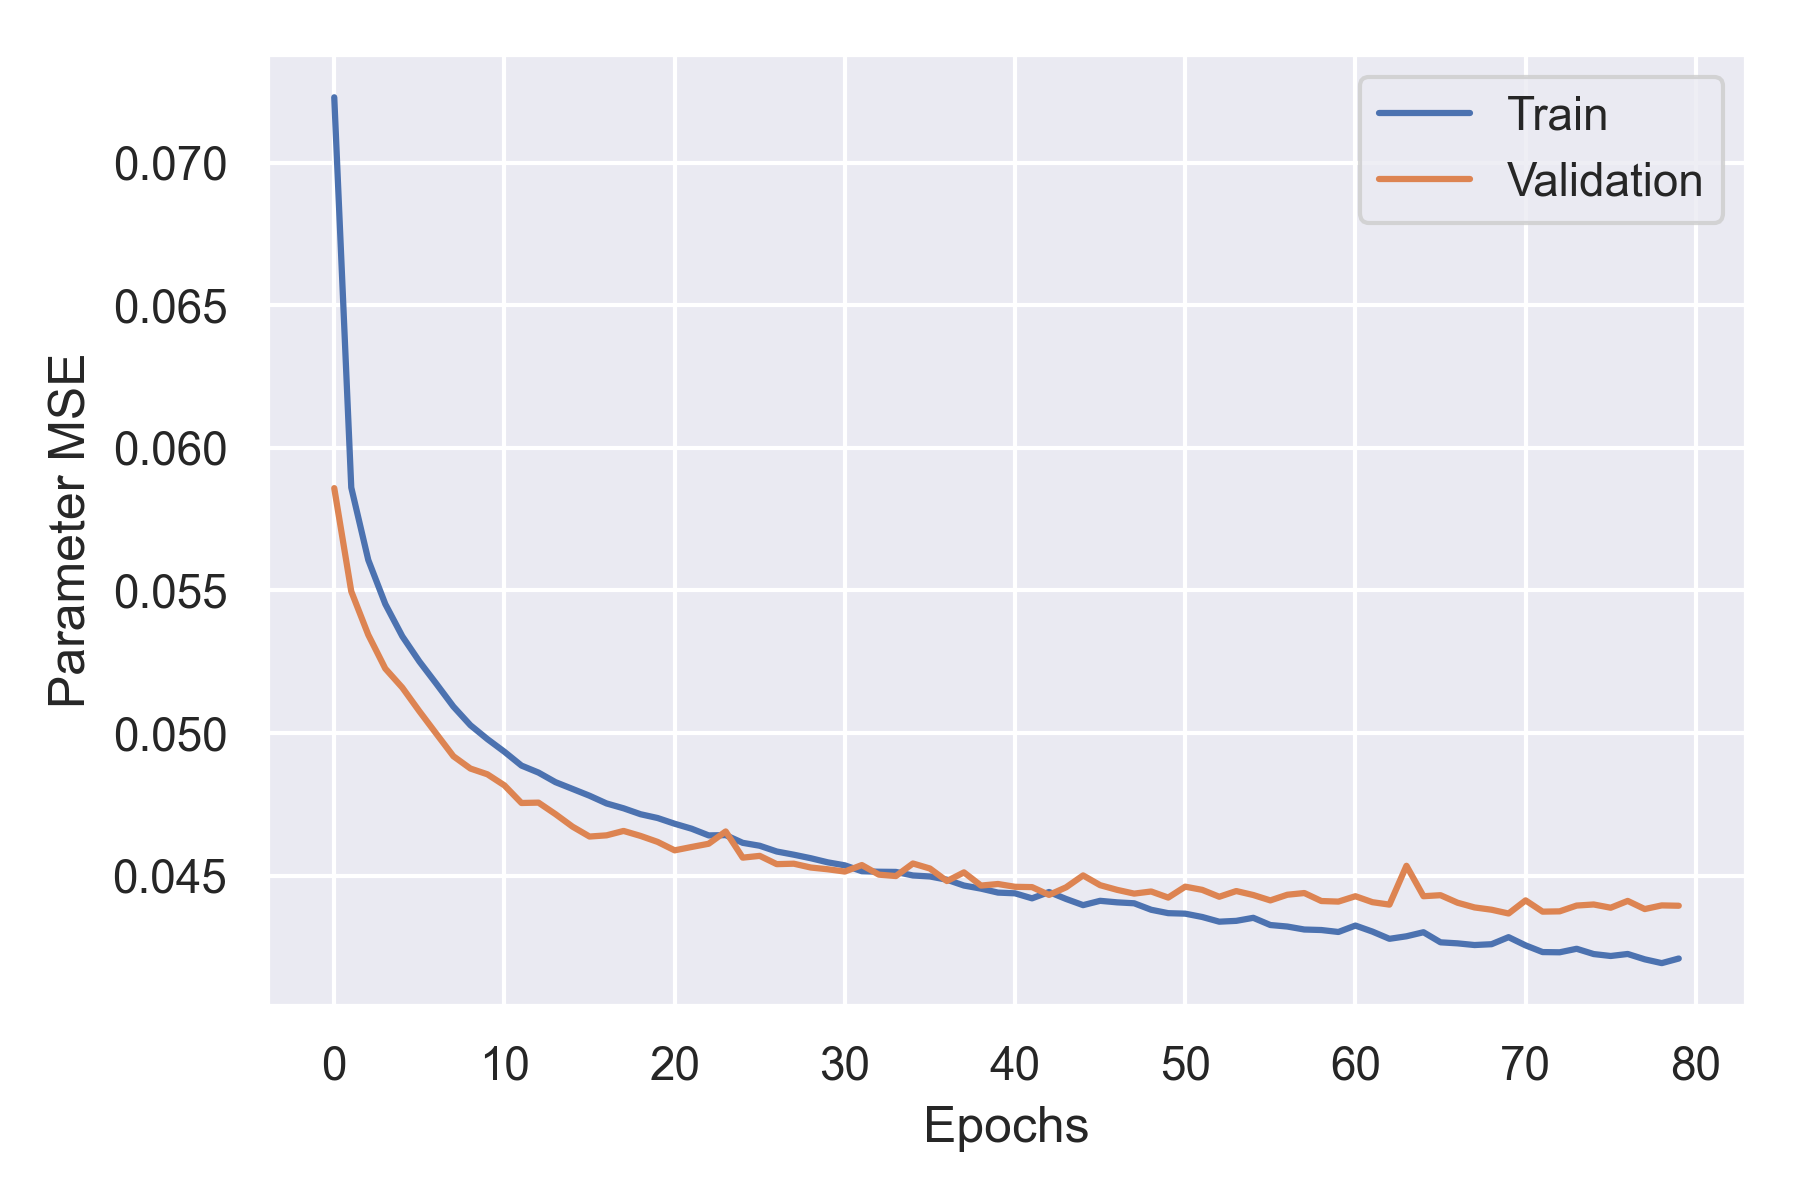
\includegraphics[width=\textwidth]{figures/inverse-synth/loss-plots/bilstm-mel.png}
        \caption{LSTM++}
    \end{subfigure}
    \begin{subfigure}[b]{0.49\textwidth}
        \centering
        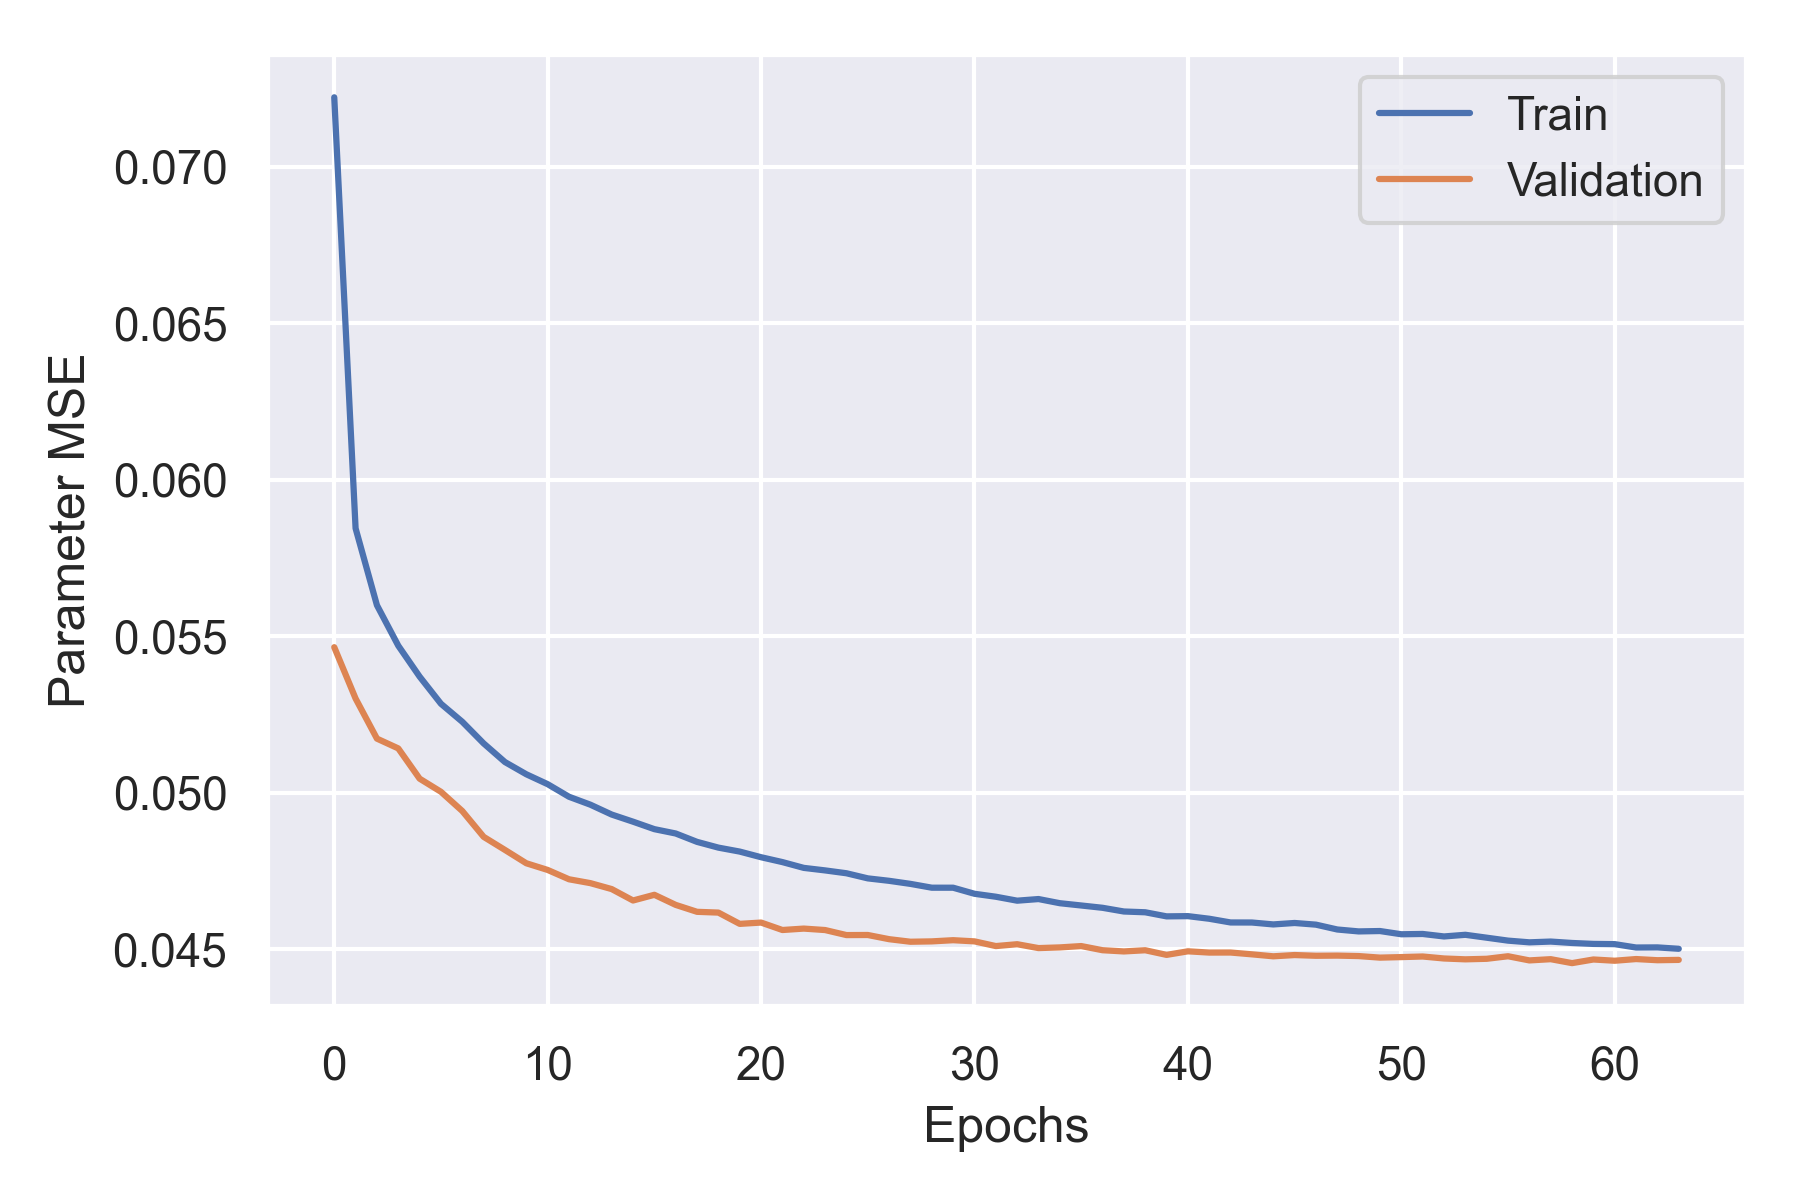
\includegraphics[width=\textwidth]{figures/inverse-synth/loss-plots/cnn-mel.png}
        \caption{CNN}
    \end{subfigure}
    \caption{Mel-Spectrogram Model Training and Validation Loss Plots}
\end{figure}